% FILE: figures/birth_life_death.tex
% Birth, life and death of a continuum

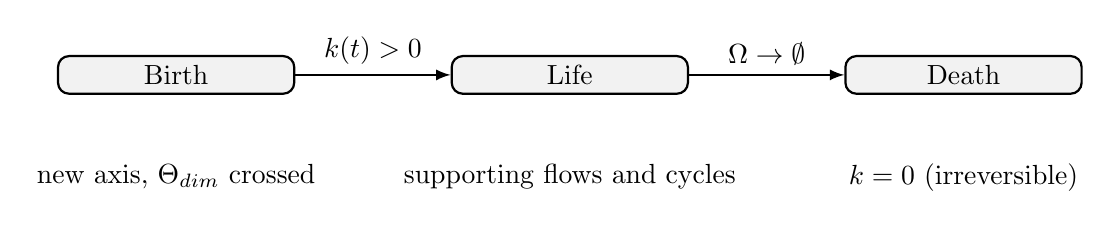
\begin{tikzpicture}[>=latex,thick]
  % States
  \node[draw, rounded corners, fill=gray!10, minimum width=3cm] (birth) at (0,0) {Birth};
  \node[draw, rounded corners, fill=gray!10, minimum width=3cm] (life)  at (5,0) {Life};
  \node[draw, rounded corners, fill=gray!10, minimum width=3cm] (death) at (10,0) {Death};

  % Arrows
  \draw[->] (birth) -- node[above] {$k(t)>0$} (life);
  \draw[->] (life)  -- node[above] {$\Omega \rightarrow \emptyset$} (death);

  % Additional labels
  \node[anchor=north] at (0,-1.0) {new axis, $\Theta_{\text{dim}}$ crossed};
  \node[anchor=north] at (5,-1.0) {supporting flows and cycles};
  \node[anchor=north] at (10,-1.0) {$k=0$ (irreversible)};
\end{tikzpicture}
